\documentclass[a4paper]{llncs}
\usepackage{graphicx}
\usepackage{url}
\usepackage{longtable}
\usepackage[latin1]{inputenc}
\usepackage{subfigure}
\usepackage{a4wide}
\urldef{\mails}\path|{ei05011,ei05028}@fe.up.pt|
\bibliographystyle{splncs}
\begin{document}
\title{Progress Report on the ``Adult Database'' analysis}
\author{Fl�vio Cruz \and Jo�o Azevedo}
\institute{Faculdade de Engenharia da Universidade do Porto\\
    Rua Dr. Roberto Frias, s/n 4200-465 Porto PORTUGAL
    \mails}
\maketitle

\begin{abstract}
Highly frequent in experimental tests related to data mining, the Adult Database
has some interesting properties which make it quite useful to test the 
efficiency of classification algorithms. This report aims to describe the Adult
Database from a statistical perspective and taking in account its support for
data mining tasks.
\end{abstract}

\section{Introduction}

\section{Data Format}

The ``Adult Database'' consists of 48842 entries of individual information of 
people gathered in a 1994 census on the United States of America. From the
global collection of data, a representative sample was collected from people
with ages between 16 and 100 and a final weight above 1.

Each entry is composed by a set of 14 attributes and a class, identifying
persons who gain more or less than 50K. The attributes and types are:

\begin{itemize}
  \item{\textbf{Age}: continuous.}
  \item{\textbf{Workclass}: categorical: [[Private], [Self-emp-not-inc], 
        [Self-emp-inc], [Federal-gov], [Local-gov], [State-gov], [Without-pay], 
        [Never-worked]]}
  \item{\textbf{FNLWGT}: continuous. Represents the final weight. People with 
        the same demographical characteristics should have the same weight.}
  \item{\textbf{Education}: ordinal: [1. [Preschool], 2. [1st-4th], 3. 
        [5th-6th], 4. [7th-8th], 5. [9th < 10th], 6. [11th < 12th], 7. 
        [HS-grad], 8. [Prof-school], 9. [Assoc-acdm], 10. [Assoc-voc], 11.
        [Some-college], 12. [Bachelors], 13. [Masters], 14. [Doctorate]]}
  \item{\textbf{Education-num}: continuous. Is a continuous representation of 
        the \textbf{Education} attribute.}
  \item{\textbf{Marital-status}: categorical: [[Married-civ-spouse], [Divorced],
        [Never-married], [Separated], [Widowed], [Married-spouse-absent],
        [Married-AF-spouse]]}
  \item{\textbf{Occupation}: categorical: [[Tech-support], [Craft-repair],
        [Other-service], [Sales], [Exec-managerial], [Prof-specialty], 
        [Handlers-cleaners], [Machine-op-inspct], [Adm-clerical], 
        [Farming-fishing], [Transport-moving], [Priv-house-serv], 
        [Protective-serv], [Armed-Forces]]}
  \item{\textbf{Relationship}: categorical: [[Wife], [Own-child], [Husband], 
        [Not-in-family], [Other-relative], [Unmarried]]}
  \item{\textbf{Race}: categorial: [[White], [Asian-Pac-Islander], 
        [Amer-Indian-Eskimo], [Other], [Black]]}
  \item{\textbf{Sex}: categorical: [[Male], [Female]]}
  \item{\textbf{Capital-gain}: continuous.}
  \item{\textbf{Capital-loss}: continuous.}
  \item{\textbf{Hours-per-week}: continuous.}
  \item{\textbf{Native-country}: categorical.}
\end{itemize}

\section{Problem Identification}

\section{Data Analysis}

The table \ref{tab:summary} summarizes the distribution of values on the studied
dataset. From a first observation, one can see that the amount of missing values
is low. On the other side, in some of the attributes, some classes have a
much higher frequency than others, as the 'united-states' native country, the
'private' workclass and the 'white' race. On the hours of work per week
attribute, there is a great amount of outliers, with some unrealistic
values, namely with values close to the 100 hours or less than 10 in individuals
with a defined occupation, as can be seen on figure \ref{fig:box_hours}.
Variables such has the capital gain and capital loss have few values above 0,
being quite specific to certain classes of individuals. The sex is also
unbalanced in the sample data, as the amount of men is more than twice the
amount of women.

It is also important to verify some correlations between variables. To that
matter, we've tested some apparent situations, such as the influence of the age,
hours of work per week and educational level on the amount gained by an
individual. The figures \ref{fig:age_plus50}, \ref{fig:education_plus50} and
\ref{fig:hpw_plus50} show that there is a tendency for older people, people with
a higher educational level and people who work a great amount of hours per week
to gain a larger amount of money.

\subsection{Association Rules}

\subsection{Clusters}

\section{Future Work}

\section{Conclusions}

\begin{thebibliography}{1}
\end{thebibliography}

\clearpage

\appendix

\section{Tables}

\begin{table}
\centering
\subtable[Age]{
       \begin{tabular}{| l | l |}
       \hline
       Min. & 17 \\
       \hline
       1st Qu. & 28 \\
       \hline
       Median & 37 \\
       \hline
       Mean & 38.58 \\
       \hline
       3rd Qu. & 48 \\
       \hline
       Max & 90 \\
       \hline
       \end{tabular}
}
\qquad\qquad
\subtable[Workclass]{        
       \begin{tabular}{| l | l |}
       \hline
       private & 22696 \\
       \hline
       self\_emp\_not\_inc & 2541 \\
       \hline
       local\_gov & 2093 \\
       \hline
       state\_gov & 1298 \\
       \hline
       self\_emp\_inc & 1116 \\
       \hline
       (Other) & 981 \\
       \hline
       NA's & 1836 \\
       \hline
       \end{tabular}
}
\qquad\qquad
\subtable[Education]{        
       \begin{tabular}{| l | l |}
       \hline
       hs\_grad & 10501 \\
       \hline
       some\_college & 7291 \\
       \hline
       bachelors & 5535 \\
       \hline
       masters & 1723 \\
       \hline
       assoc\_voc & 1382 \\
       \hline
       11th & 1175 \\
       \hline
       (Other) & 5134 \\
       \hline
       \end{tabular}
}
\qquad\qquad
\subtable[Marital Status]{        
       \begin{tabular}{| l | l |}
       \hline
       divorced & 4443 \\
       \hline
       married\_af\_spouse & 23 \\
       \hline
       married\_civ\_spouse & 14976 \\
       \hline
       married\_spouse\_absent & 418 \\
       \hline
       never\_married & 10683 \\
       \hline
       separated & 1025 \\
       \hline
       widowed & 993 \\
       \hline
       \end{tabular}
}
\qquad\qquad
\subtable[Occupation]{        
       \begin{tabular}{| l | l |}
       \hline
       prof\_specialty & 4140 \\
       \hline
       craft\_repair & 4099 \\
       \hline
       exec\_managerial & 4066 \\
       \hline
       adm\_clerical & 3770 \\
       \hline
       sales & 3650 \\
       \hline
       (Other) & 10993 \\
       \hline
       NA's & 1843 \\
       \hline
       \end{tabular}
}
\qquad\qquad
\subtable[Relatonship]{        
       \begin{tabular}{| l | l |}
       \hline
       husband & 13193 \\
       \hline
       not\_in\_family & 8305 \\
       \hline
       other\_relative & 981 \\
       \hline
       own\_child & 5068 \\
       \hline
       unmarried & 3446 \\
       \hline
       wife & 1568 \\
       \hline
       \end{tabular}
}
\qquad\qquad
\subtable[Race]{        
       \begin{tabular}{| l | l |}
       \hline
       amer\_indian\_eskimo & 311 \\
       \hline
       asian\_pac\_islander & 1039 \\
       \hline
       black & 3124 \\
       \hline
       other & 271 \\
       \hline
       white & 27816 \\
       \hline
       \end{tabular}
}
\qquad\qquad
\subtable[Sex]{        
       \begin{tabular}{| l | l |}
       \hline
       female & 10771 \\
       \hline
       male & 21790 \\
       \hline
       \end{tabular}
}
\qquad\qquad
\subtable[Capital Gain]{        
       \begin{tabular}{| l | l |}
       \hline
       Min. & 0 \\
       \hline
       1st Qu. & 0 \\
       \hline
       Median & 0 \\
       \hline
       Mean & 1078 \\
       \hline
       3rd Qu. & 0 \\
       \hline
       Max. & 99999 \\
       \hline
       \end{tabular}
}
\qquad\qquad
\subtable[Capital Loss]{        
       \begin{tabular}{| l | l |}
       \hline
       Min. & 0 \\
       \hline
       1st Qu. & 0 \\
       \hline
       Median & 0 \\
       \hline
       Mean & 87.3 \\
       \hline
       3rd Qu. & 0 \\
       \hline
       Max. & 4356 \\
       \hline
       \end{tabular}
}
\qquad\qquad
\subtable[Hours Per Week]{        
       \begin{tabular}{| l | l |}
       \hline
       Min. & 1 \\
       \hline
       1st Qu. & 40 \\
       \hline
       Median & 40 \\
       \hline
       Mean & 40.44 \\
       \hline
       3rd Qu. & 45 \\
       \hline
       Max. & 99 \\
       \hline
       \end{tabular}
}
\qquad\qquad
\subtable[Native Country]{        
       \begin{tabular}{| l | l |}
       \hline
       United States & 29170 \\
       \hline
       Mexico & 643 \\
       \hline
       Philippines & 198 \\
       \hline
       Germany & 137 \\
       \hline
       Canada & 121 \\
       \hline
       (Other) & 1709 \\
       \hline
       NA's & 583 \\
       \hline
       \end{tabular}
}
\qquad\qquad
\subtable[Plus 50]{        
       \begin{tabular}{| l | l |}
       \hline
       No & 24720 \\
       \hline
       Yes & 7841 \\
       \hline
       \end{tabular}
}
\caption{Summary of the value distribution in the database}
\label{tab:summary}
\end{table}

\clearpage

\section{Figures}

\begin{figure}
\centering
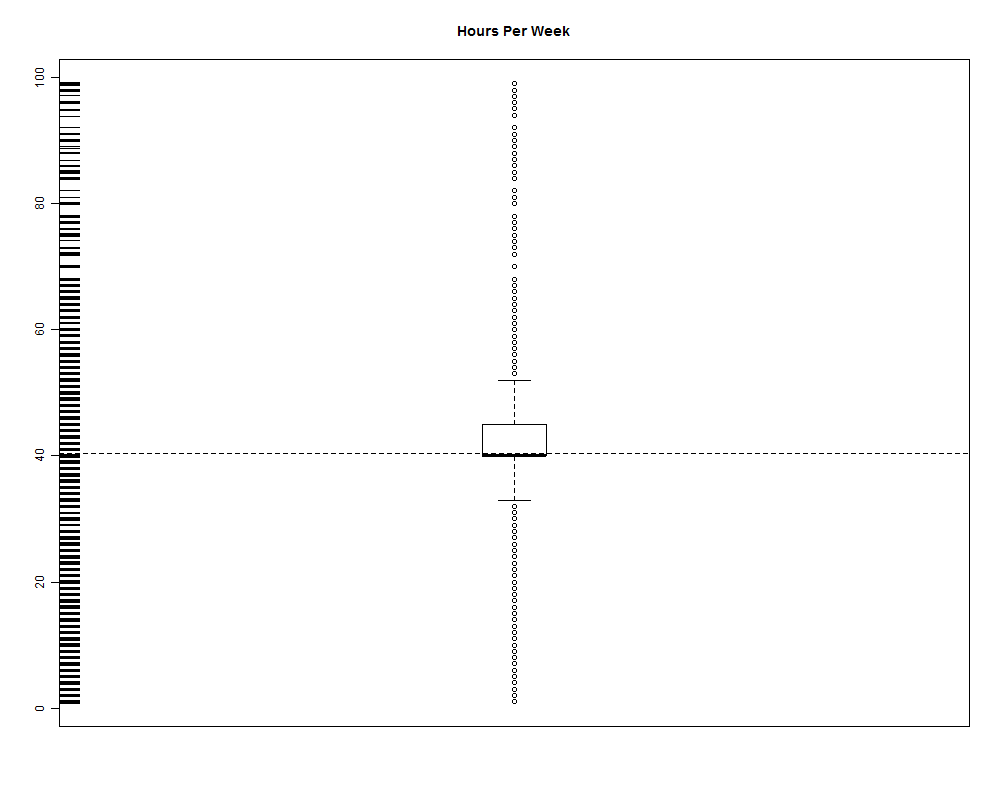
\includegraphics[width=10cm]{boxplot_hours_per_week.png}
\caption{Boxplot of the hours per week variable}
\label{fig:box_hours}
\end{figure}

\begin{figure}
\centering
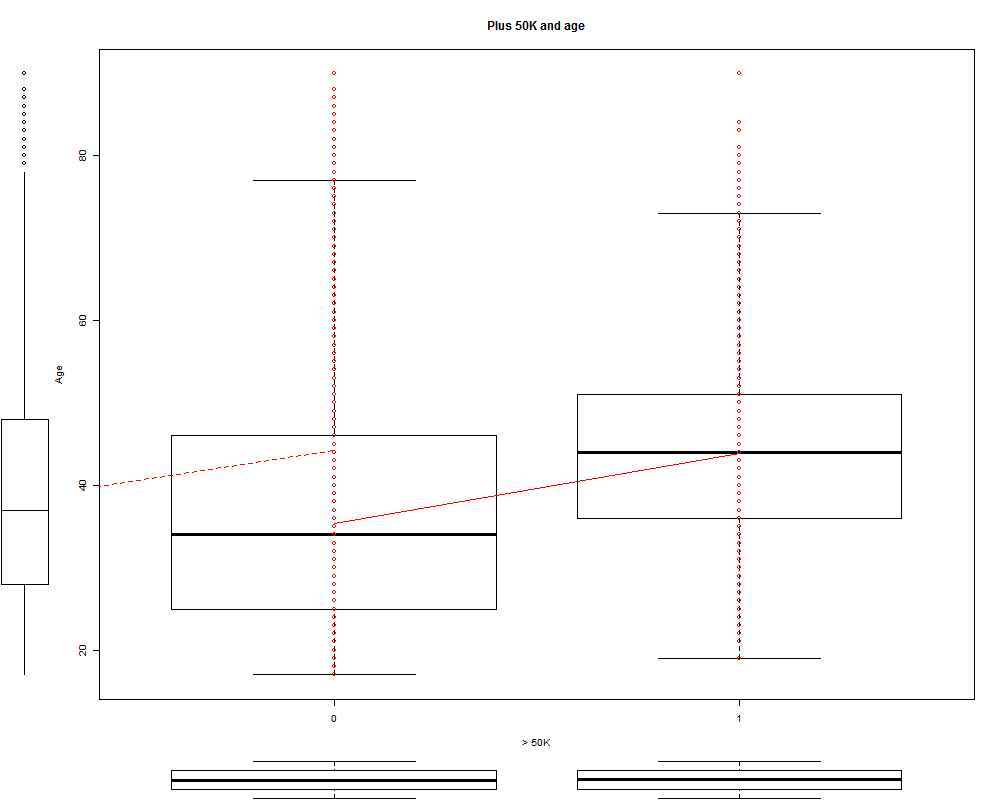
\includegraphics[width=10cm]{plot_plus_50_age.png}
\caption{Boxplot of the individuals' age, for each class of gain}
\label{fig:age_plus50}
\end{figure}

\begin{figure}
\centering
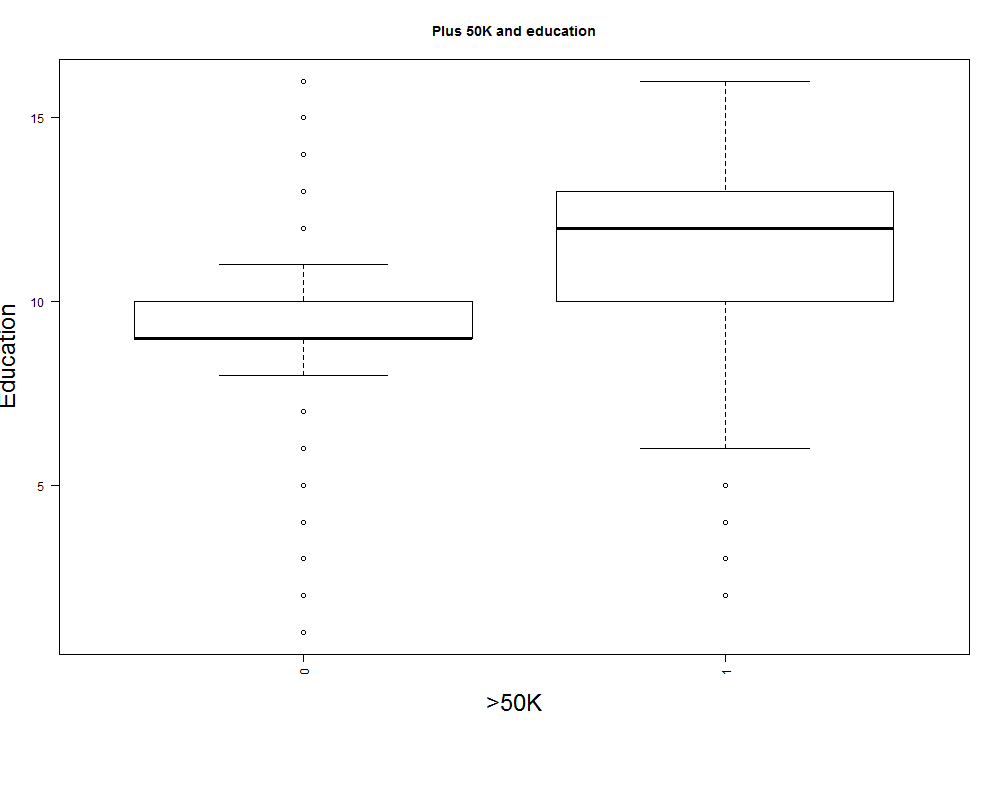
\includegraphics[width=10cm]{plot_plus_50_education_num.png}
\caption{Boxplot of the individuals' education level, for each class of gain}
\label{fig:education_plus50}
\end{figure}

\begin{figure}
\centering
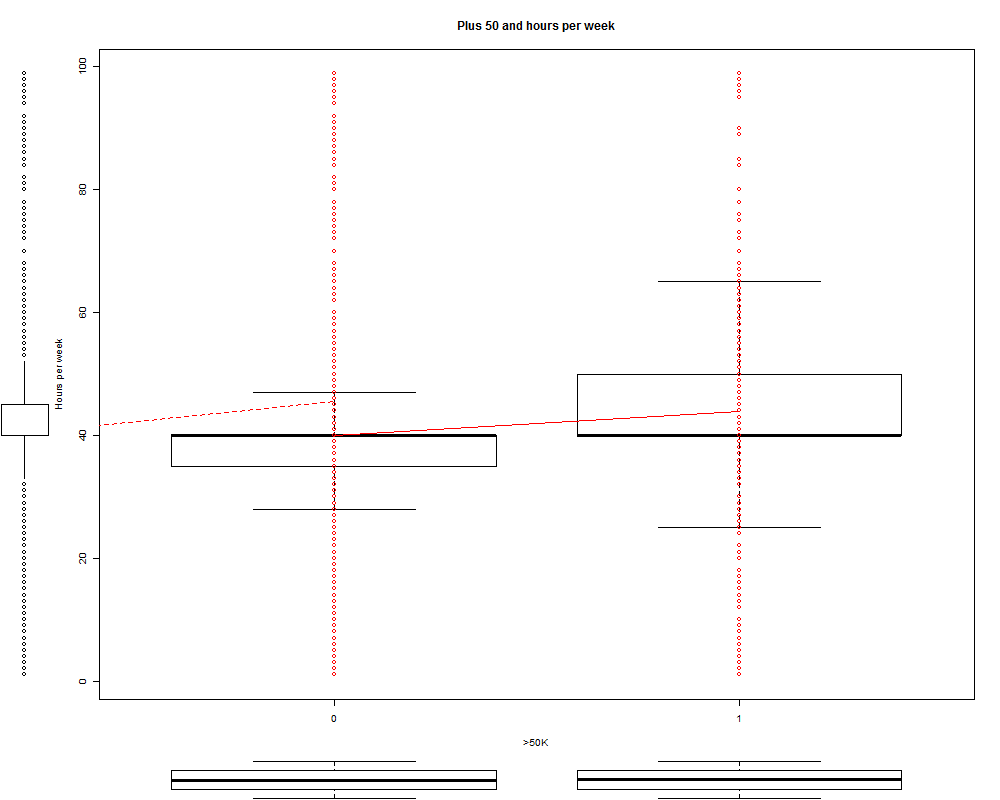
\includegraphics[width=10cm]{plot_plus_50_hpw.png}
\caption{Boxplot of the individuals' hours of work per week, for each class of 
gain}
\label{fig:hpw_plus50}
\end{figure}

\end{document}
